\section{Reuniones iniciales con los clientes}

La reunión inicial fue con Juan Francisco Sanjuan Estrada donde me explicó los distintos objetivos que se tenía pensado para la aplicación y los puntos de vista de los técnicos. La organización, gestión y préstamos del inventario se realizaba mediante la utilización de hojas de cálculo.
\\Dentro de las hojas de cálculo se hacía un detallado exhaustivo del objeto y también se indicaba su ubicación actual dentro del Edificio Científico Técnico III.
\\El problema es que esto no estaba tan organizado como parecía en un principio debido a que la gestión no la realizaba únicamente un técnico sino que eran tres. Es decir, había tres filosofías distintas a la hora de ir gestionando una parte dle inventariado del Departamento de Informática.
\\Después de estas aclaraciones Juan me comentó que no tenían un diseño en mente en el Departamento por lo que las propuestas iniciales de diseño iban a ser libres siempre y cuando se satisfacieran los requisitos principales de esta como la adición y eliminación del inventario y la concesión de préstamos.
\\\\Luego de esta primera reunión acordamos en que podría visualizar los archivos Excel de los técnicos. Estos me compartieron sus ficheros y desde ahí pude empezar a realizar la definición de los diferentes campos que irían ligados a cada tabla en la base de datos. Desde esa primera definición de campos se haría una propuesta inicial.
\\La propuesta inicial fue esta:

\begin{figure}\resizebox{
    \linewidth}{!}{
    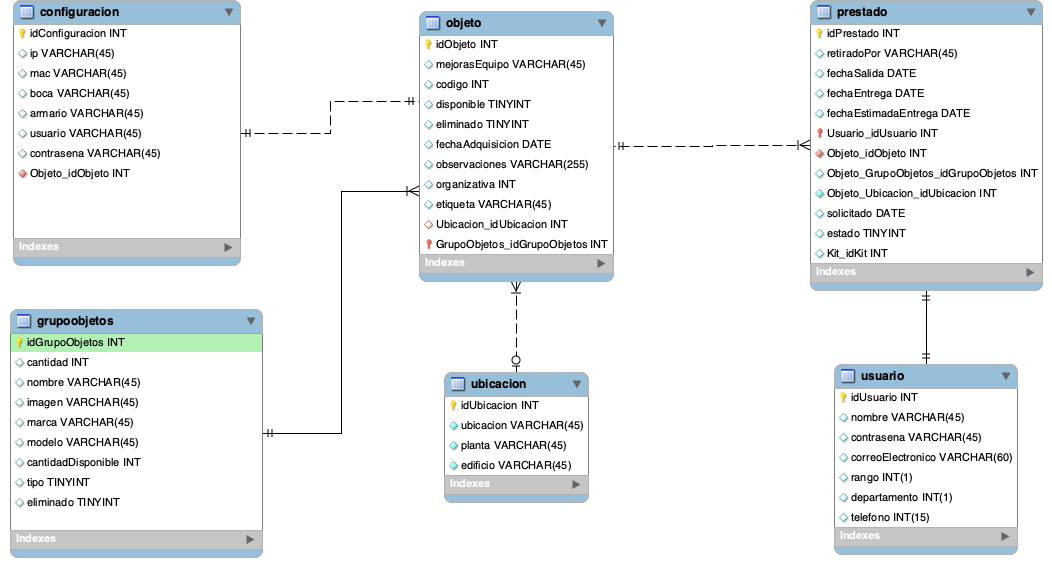
\includegraphics{db_old_design.png}
    }
    \caption{Diseño principal de la base de datos}
\end{figure}

La lógica de la aplicación consistiría en generar un grupoobjetos de un determinado tipo, inventario o fungible, 1 o 0. Dentro de este se contendrían objetos que irían vinculados a una ubicación. También los objetos irían vinculados a una posible configuración.
\\Esta configuración ¿para qué sirviría? Resulta que los técnicos aparte de manejar el inventariado disponible en la universidad también manejan las claves y accesos a esos determinados objetos, como puede ser el armario donde se ubiquen, sus direcciones mac o ip, las bocas de conexión con las regletas y más.
\\Este objeto tendría la posibilidad de tener varios préstamos, aunque es verdad que sería uno activo por persona, siempre dejando un registro de los anteriores usos que se hayan realizado del mismo. Este préstamo tendría que ir ligado obligatoriamente a un usuario. Contiene un campo de ``retiradoPor'' en el caso de que un docente o investigador quiera realizar un préstamo para su alumno.
\\\\La propuesta inicial fue aceptada por el grupo de los técnicos y por el director del proyecto así que podíamos continuar hacia adelante. Más adelante se realizaron unas modificaciones en los datos que manejarían los objetos por lo que las columnas de la tabla son las definitivas.
\\Preparé las propuestas iniciales de diseño mediante la utilización de la herramiento de Adobe XD. El aprendizaje de la herramienta es rápido y fácil de usar, aparte de que ya la había empezado a utilizar unos años atrás. Adobe XD le dió un toque de frescura y profesionalidad a las propuestas de diseño.
\\Las propuestas iniciales fueron ligadas a un diseño móvil ya que desde el primer momento se buscó que fuera responsive el sitio web. Esto influyó luego a la hora de realizar el diseño ya que se basó en un funcionamientos de ``cards'', es decir, componentes web con forma de carta y con fácil adaptabilidad a diseños móviles.
\\El esquema de navegación de la propuesta inicial nos quedaría tal que así:

\begin{figure}\resizebox{
    \linewidth}{!}{
    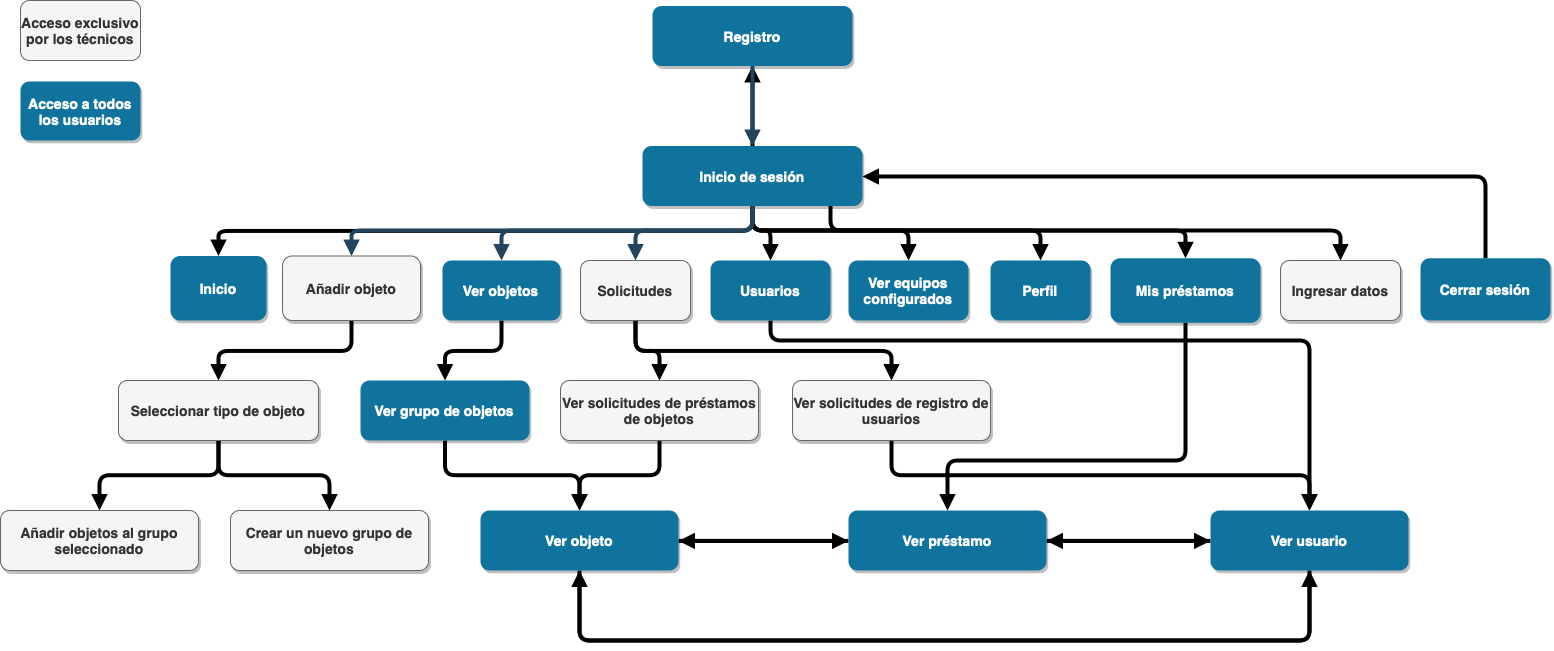
\includegraphics{flujo_de_navegacion.png}
    }
    \caption{Diseño principal del sistema de navegación}
\end{figure}

\subsection{Inicio de sesión y registro}

El registro del usuario no conllevaba un registro instantáneo del mismo ya que este tiene que ser dado de alta por un técnico del sistema.

\begin{figure}
    \begin{center}
        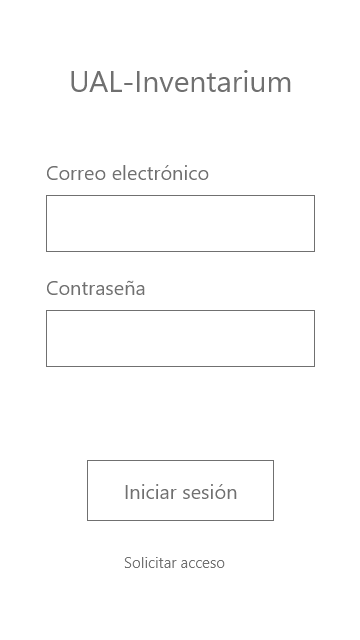
\includegraphics[scale=0.5]{web_design_adobe_xd/inicio_de_sesion.png}
        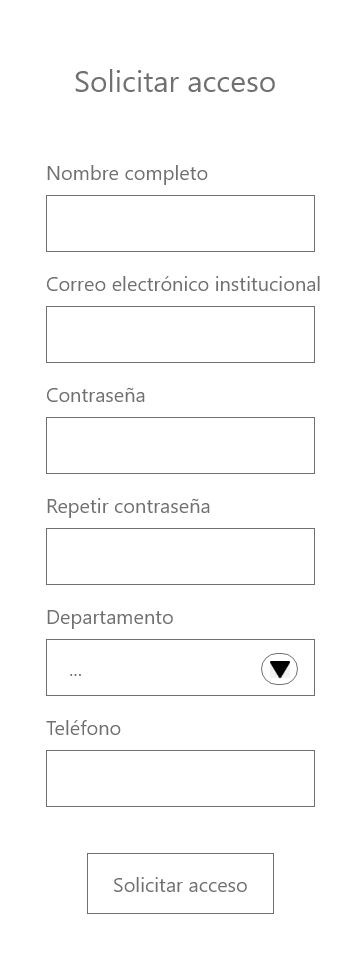
\includegraphics[scale=0.4]{web_design_adobe_xd/registro.png}
        \caption{Diseño del inicio de sesión y del registro}
    \end{center}
\end{figure}

Dentro del inicio de sesión vemos un campo interesante a considerar y es el de departamento. Una de las solicitudes que hizo el director del proyecto era poder agrupar a los usuarios dentro de departamentos. En este caso refiriéndose a dentro del personal docente e investigador que pertenecen al Departamento de Informática.
\\Los valores del departamento en la base de datos pueden ser los siguientes:

\begin{itemize}
    \item 0 = Departamento de informática (valor por defecto)
    \item 1 = Ingeniería de sistemas y automática
    \item 2 = Lenguaje y sistemas informáticos
    \item 3 = Ciencias de la computación e inteligencia artificial
    \item 4 = Arquitectura y tecnología de computadores
\end{itemize}

Otro campo para comprobar es el del correo electrónica institucional teniendo que ser este con la extensión \textbf{@inlumine.ual.es} o \textbf{@ual.es}.

\subsection{Barra de navegación}

La barra de navegación vertical tuvo una pequeña modificación que era incorporar una pequeña sección de inicio donde aparecieran información pertinente y relevante para el usuario. Esto será explicado más adelante en la parte de desarrollo.

\begin{figure}
    \begin{center}
        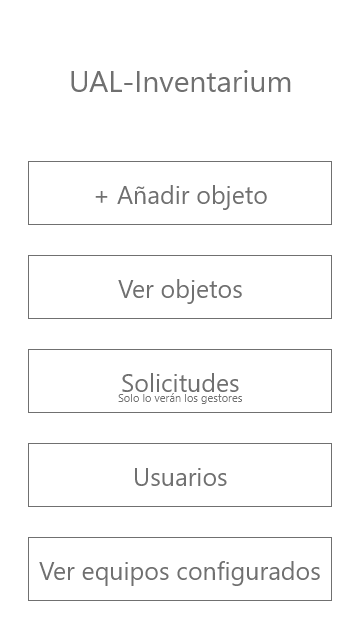
\includegraphics[scale=0.5]{web_design_adobe_xd/menu_principal.png}
        \caption{Diseño de la barra lateral de búsqueda}
    \end{center}
\end{figure}

Dentro de ella podemos ver cinco apartados que derivan en cinco??? componentes visuales:

\begin{itemize}
    \item Añadir objeto: un acceso rápido donde poder añadir objetos dentro de grupos de objetos. Sección de menú solo visible para los técnicos.
    \item Ver objetos: apartado donde se visualizan los grupos de objetos, que contienen tanto el inventariado, fungibles y kits.
    \item Solicitudes: un menú donde se visualizan las solicitudes tanto de alta de usuarios como de objetos que le puedan llegar a los técnicos.
    \item Usuarios: componente visual donde cargan los usuarios registrados que hay dentro de la aplicación.
    \item Ver equipos configurados: aquí cargan únicamente objetos a los que se les haya aplicado una configuración. En caso de que no, no aparecerían.
\end{itemize}

\subsection{Añadir objeto}
\begin{figure}
    \begin{center}
        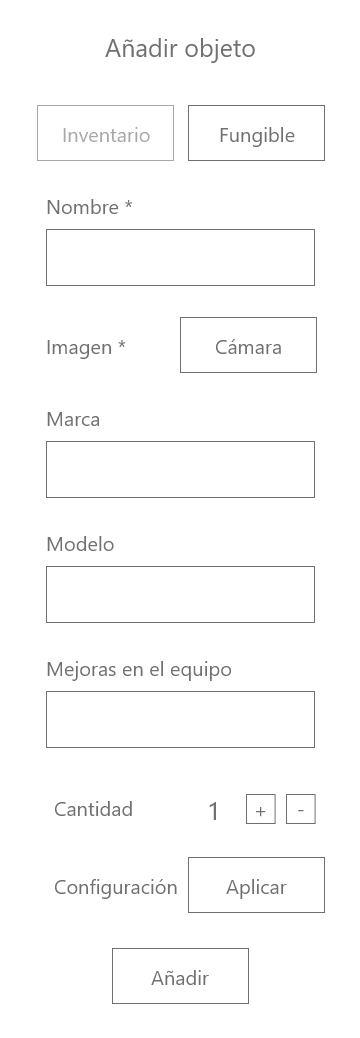
\includegraphics[scale=0.5]{web_design_adobe_xd/add_fungible.png}
        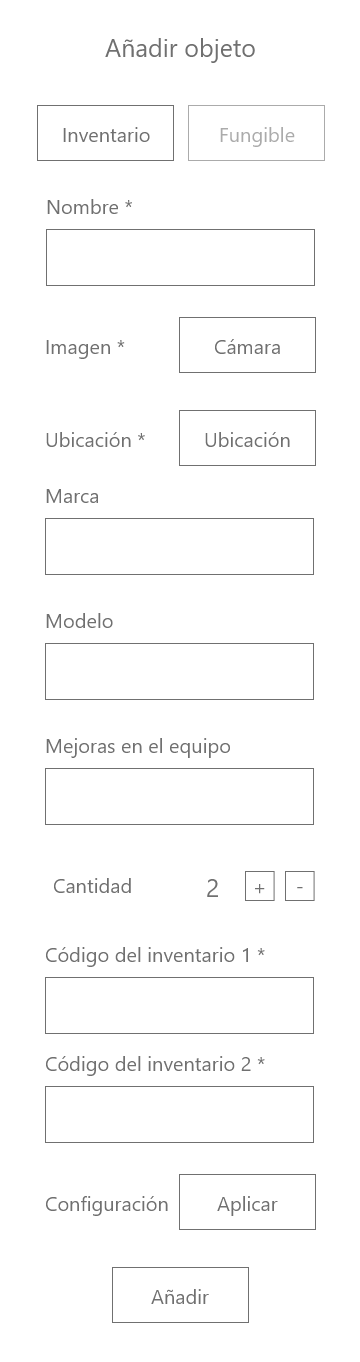
\includegraphics[scale=0.4]{web_design_adobe_xd/add_inventario.png}
        \caption{Diseño de la característica para poder añadir fungibles e inventarios}
    \end{center}
\end{figure}

